\subsection{Kobling fra database til objekt}
For at mappe databasen til objekter anvendes property mapping. Property mapping er simpelt sagt hvor tabelerne er koblet til modelklasserne og kolonerne er koblet til attributterne. Via et Data Structure Diagram illustreres den fysiske data model. Her kan hele diagrammet ses på figur \ref{fig:DSD}.

\begin{figure}[H]
    \centering
    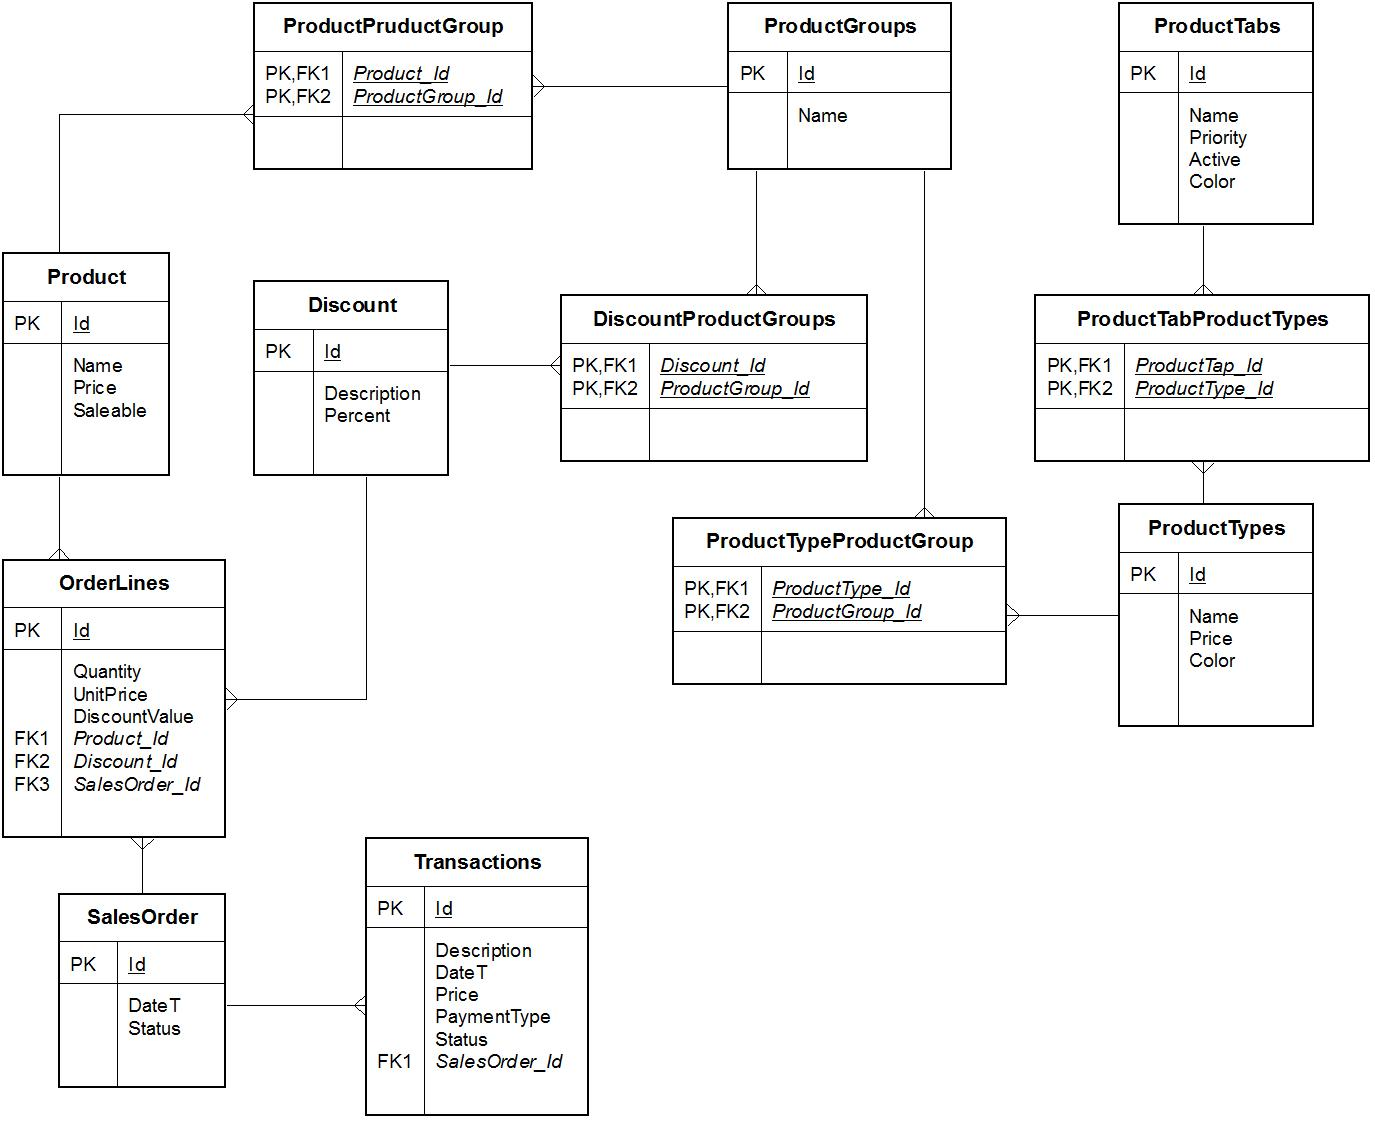
\includegraphics[width=1\textwidth]{N+1/DataView/DabDSD}
    \caption{fysisk data model}
    \label{fig:DSD}
\end{figure}

For at gøre det mere overskueligt, vil koblingen af den fysiske data model og klasse modellerne blive delt op i flere diagrammer. Hertil vil der være nogle overordnede forklaringer på hvorfor databasen er blevet designet som den er og hvordan det er løst med modelklasserne. Her kan hele pakken for model klasserne ses på figur \ref{fig:Models_CLASS}.

\subsubsection{Transaction og SalesOrder}
På figur \ref{fig:Mapping_TS} ses koblingen af tabellen Transaction\fxnote{glossery} og SalesOrder\fxnote{glossery} tabellerne

\begin{figure}[H]
    \centering
    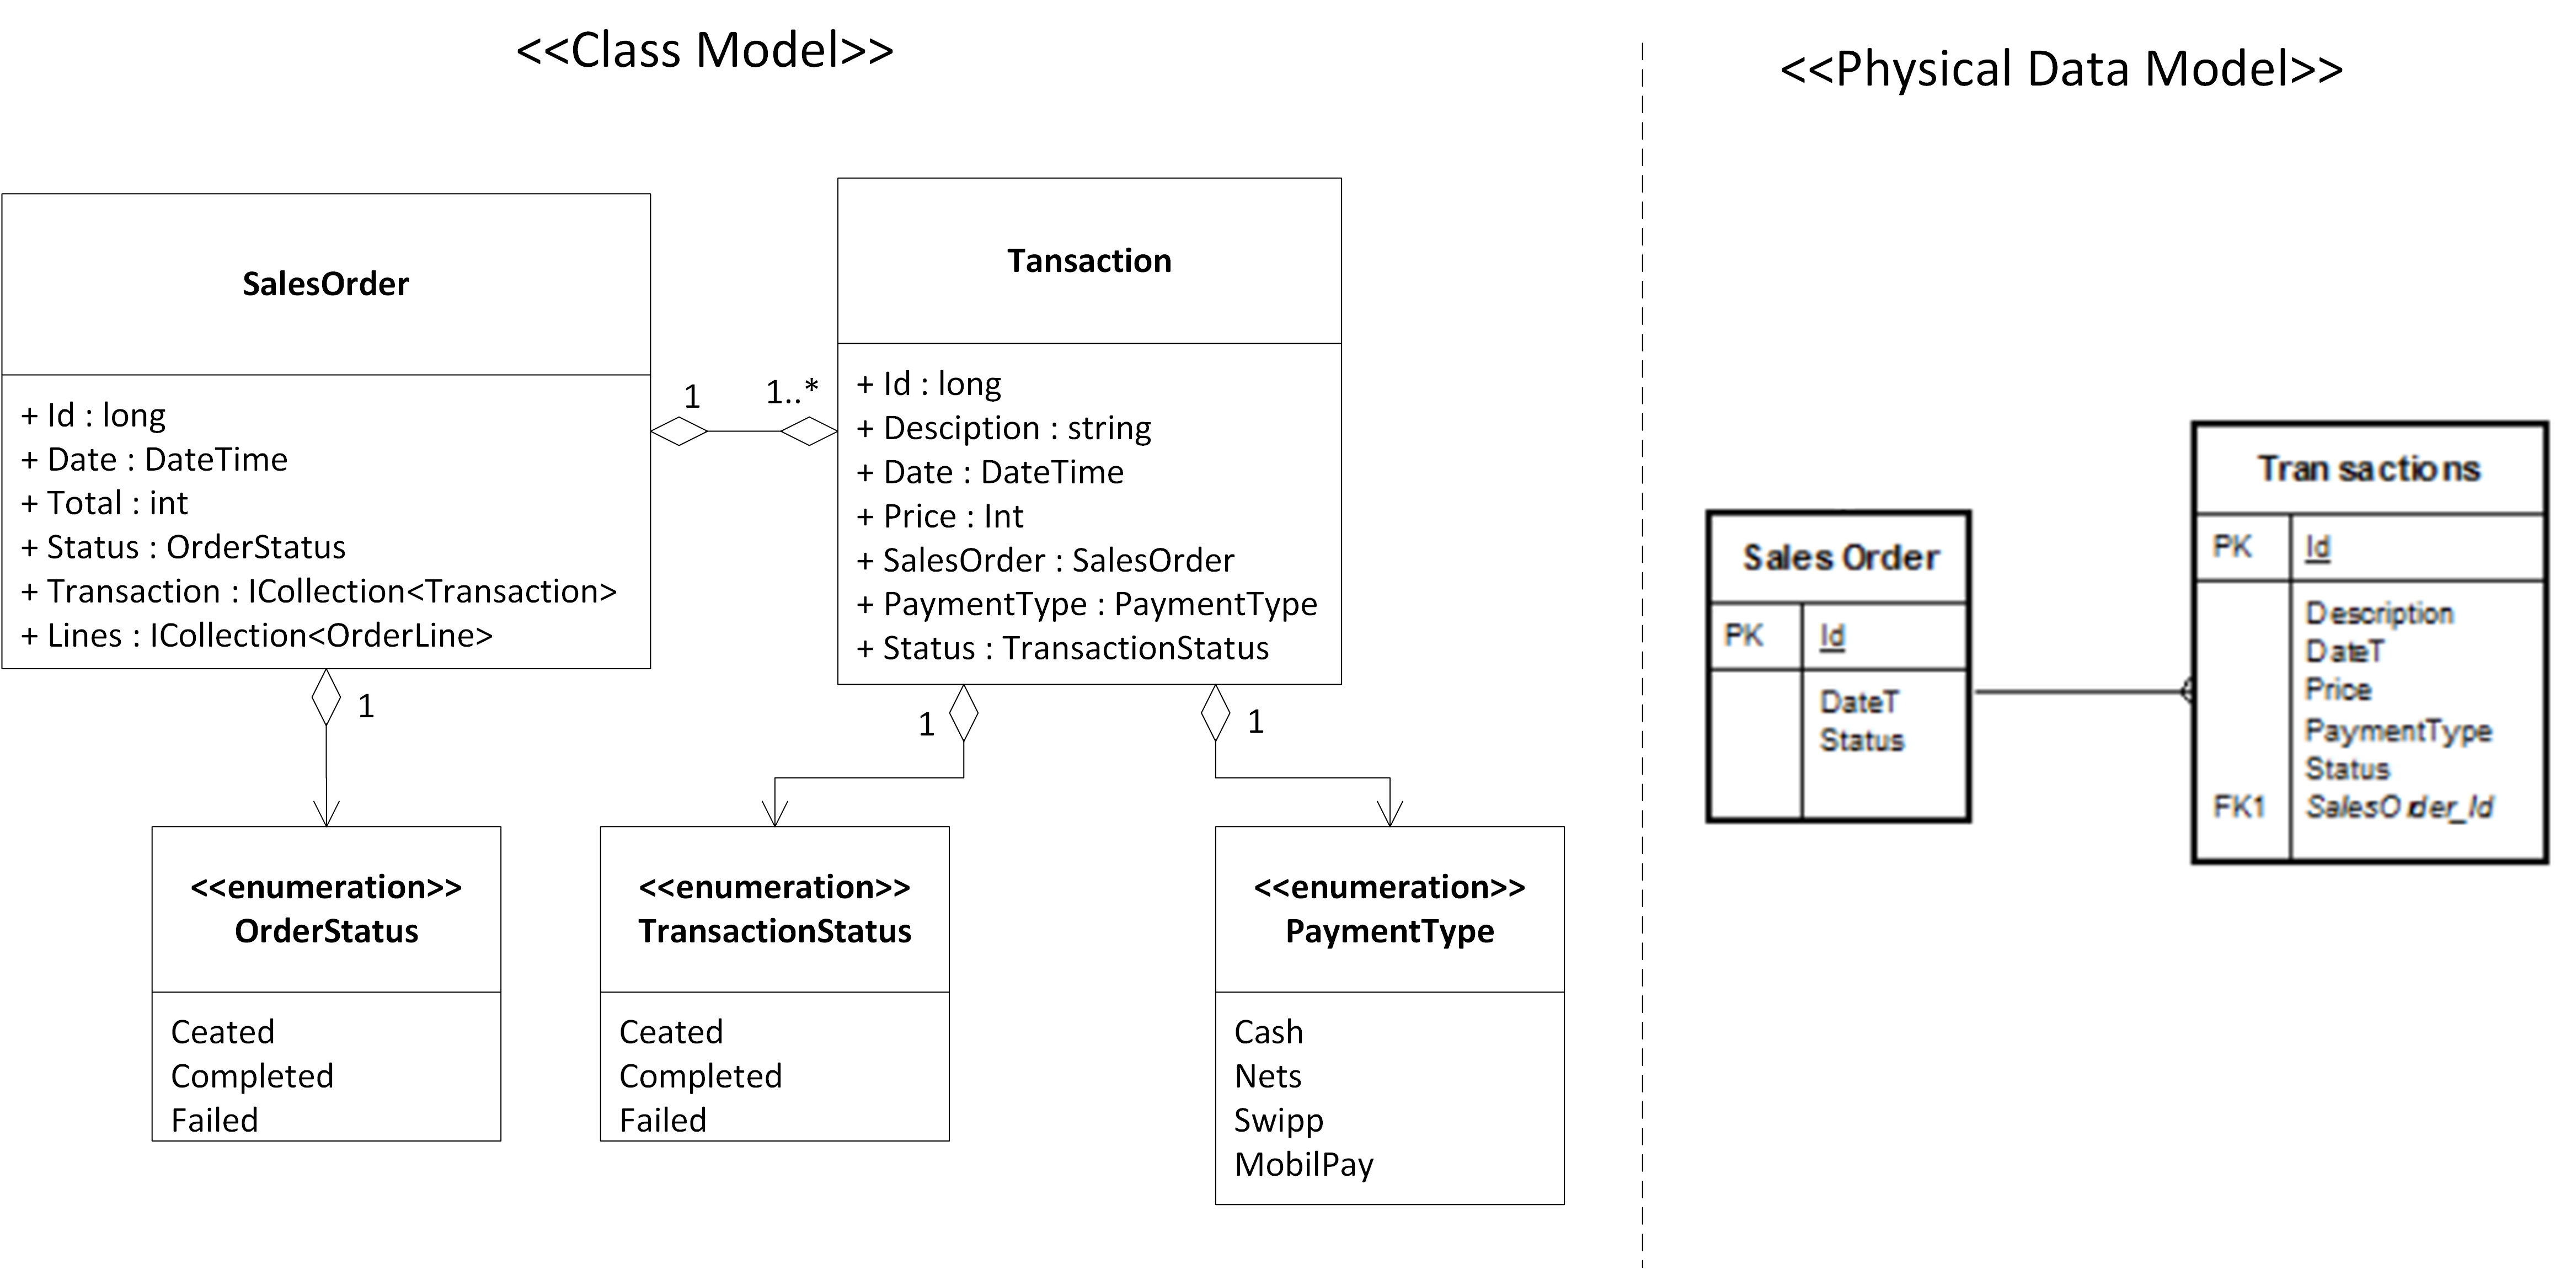
\includegraphics[width=1\textwidth]{N+1/DataView/mapping/Mapping1}
    \caption{kobling af Transaction og SalesOrder}
    \label{fig:Mapping_TS}
\end{figure}

Her kan det ses, at attributterne i klasse modellen minder meget om kolonerne i tabellerne med nogle få forskelle. En lille ting man kan lægge mærke til er at PaymentType\fxnote{glossery} og Status\fxnote{glossery} er gemt som integers, da deres egentlige navne er gemt i nogle enums inde i C\# koden. 
\newline\newline
Hvis man ser på den fysiske data model, kan det ses at Sales order har et one-to-many forhold, da det skal være muligt for kunden at betale med flere betalingsformer under et salg. For at oversætte dette til klasse modelen har SalesOrder en ICollection af Transactions, så man ud fra sales kan tilgå alle de Transaktioner der har været brugt. 

\subsubsection{OrderLine}
På figur \ref{fig:Mapping_Orderline} ses kobling af OrderLine, Product, Discount og SalesOrder\fxnote{glossery}. 

\begin{figure}[H]
    \centering
    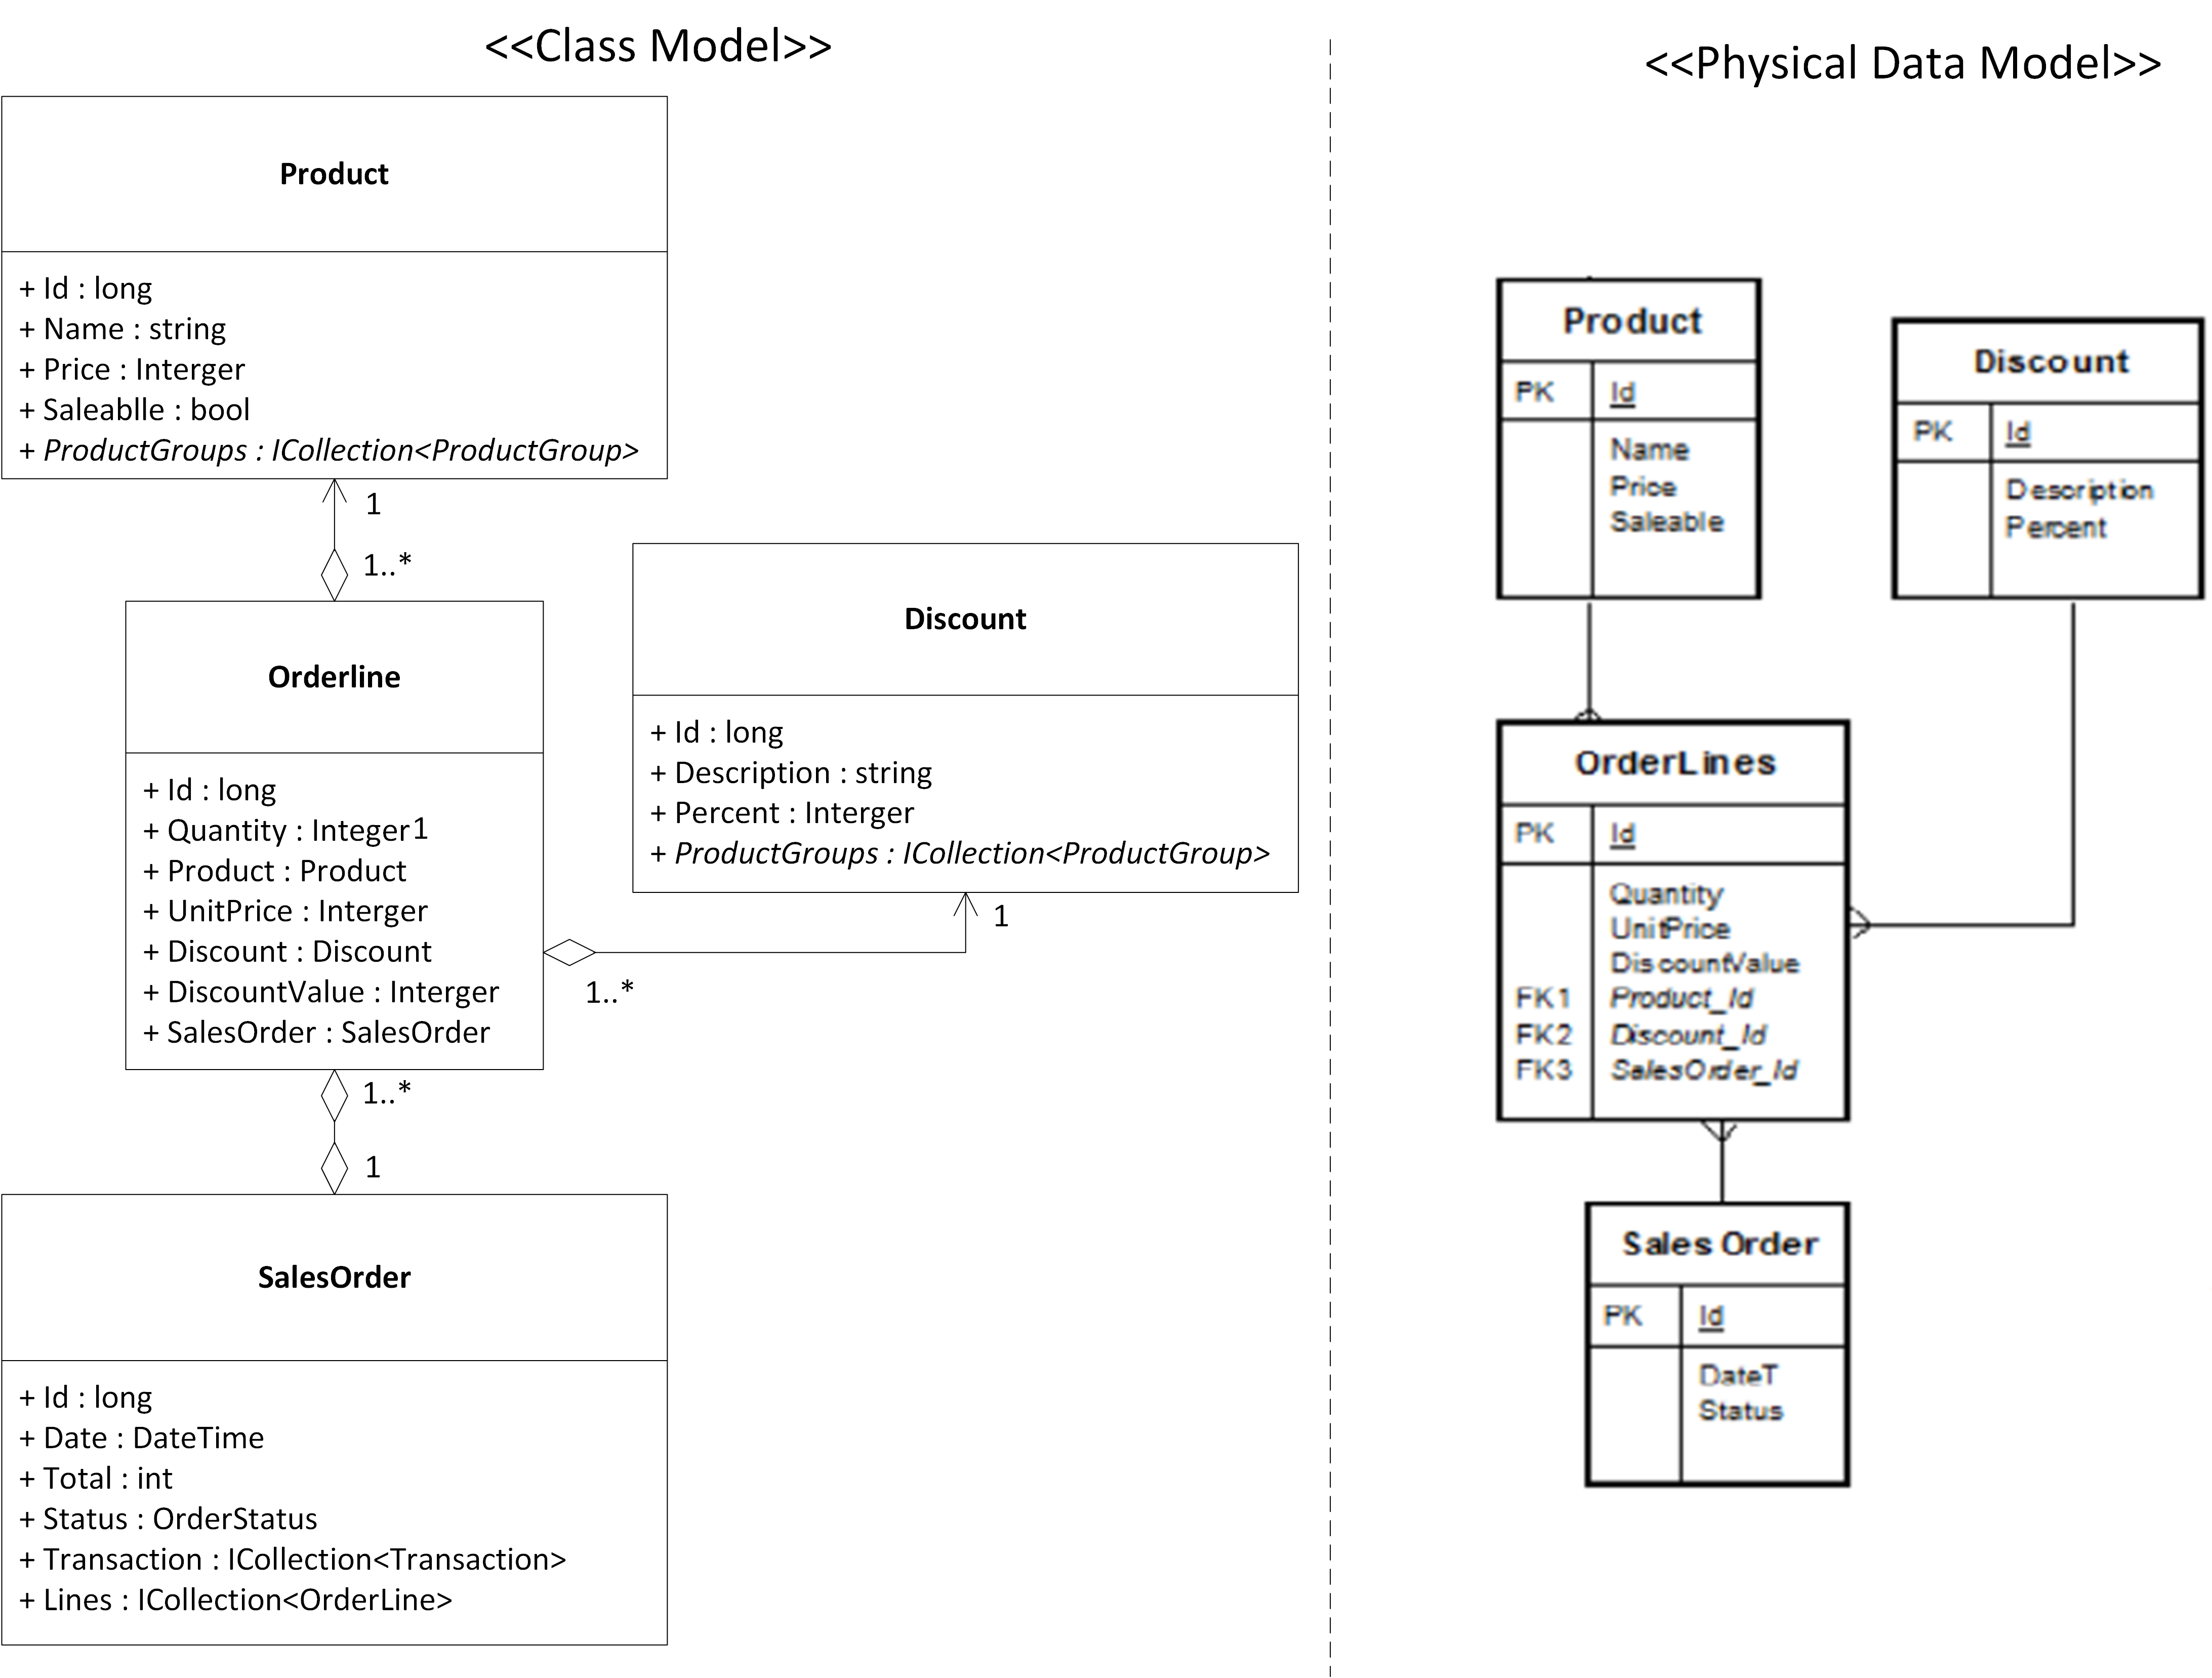
\includegraphics[width=1\textwidth]{N+1/DataView/mapping/Mapping2}
    \caption{Kobling af Orderline}
    \label{fig:Mapping_Orderline}
\end{figure}

\texttt{OrderLine} er sat op så denne skal fremstå som køb af en vare. Da Discounts kan anvendes flere gange, og der selvfølgeligt kan blive købt mere af det samme Product, skal det være muligt for Discount og Product at være indeholdt i flere \texttt{OrderLines}. Derfor er der lavet et one-to-many forhold mellem OrderLine og Product/Disccount, og da dette er løst med en fremmednøgle i den fysiske database, har klasse modellen bare fået en attribut med typen Product og Discount. 
\newline\newline
SalesOrder indholder alle de OrdeLines der er lavet til et køb. Derfor er de sat op som en one-to-many tabel, og her har OrderLine en fremmednøgle til SalesOrder og SalesOrder har en ICollection af OrderLines så de direkte kan tilgåes ud fra den. 

\subsubsection{ProductGroup}
På figur \ref{fig:Mapping_ProductGroup} ses kobling af Product, Discount og ProductGroup
\begin{figure}[H]
    \centering
    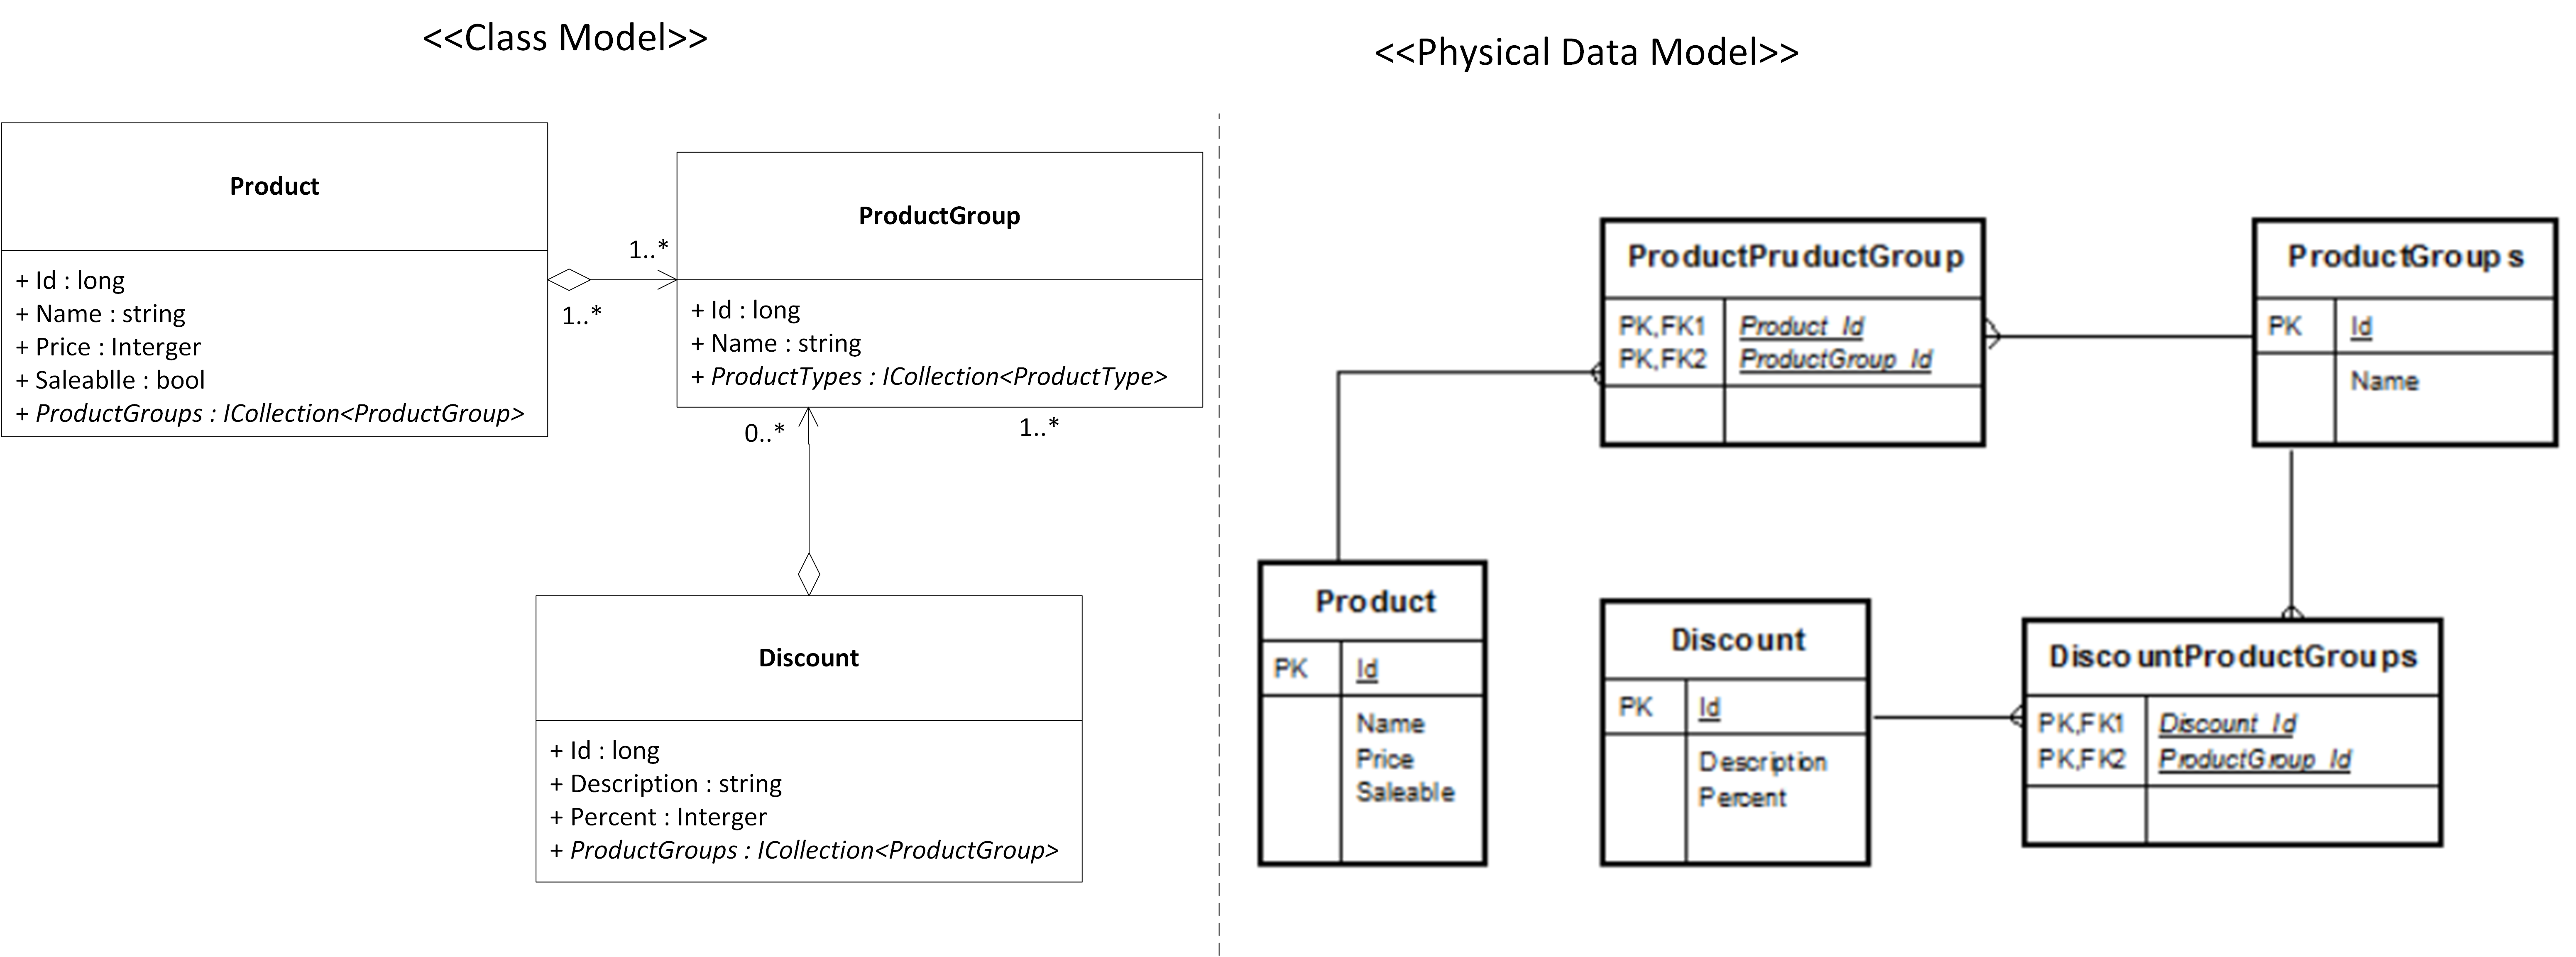
\includegraphics[width=1\textwidth]{N+1/DataView/mapping/Mapping3}
    \caption{Kobling af ProductGroup}
    \label{fig:Mapping_ProductGroup}
\end{figure}

På den fysiske data model kan det ses at Product og Discount har et many-to-many forhold med ProductGroup, da der både kan være flere Producter i en Productgrouppe, men et Product kan også være indeholdt i flere ProductGroups og det samme gælder på Discount. Dette er løst i klassemodellen ved at give en ICollection af ProductGroups til Discount og Product. 

\subsection{ProductType og ProductTap}

På figur \ref{fig:Mapping_ProductTap_Type} ses kobling af ProductTap, ProductType og ProductGroup

\begin{figure}[H]
    \centering
    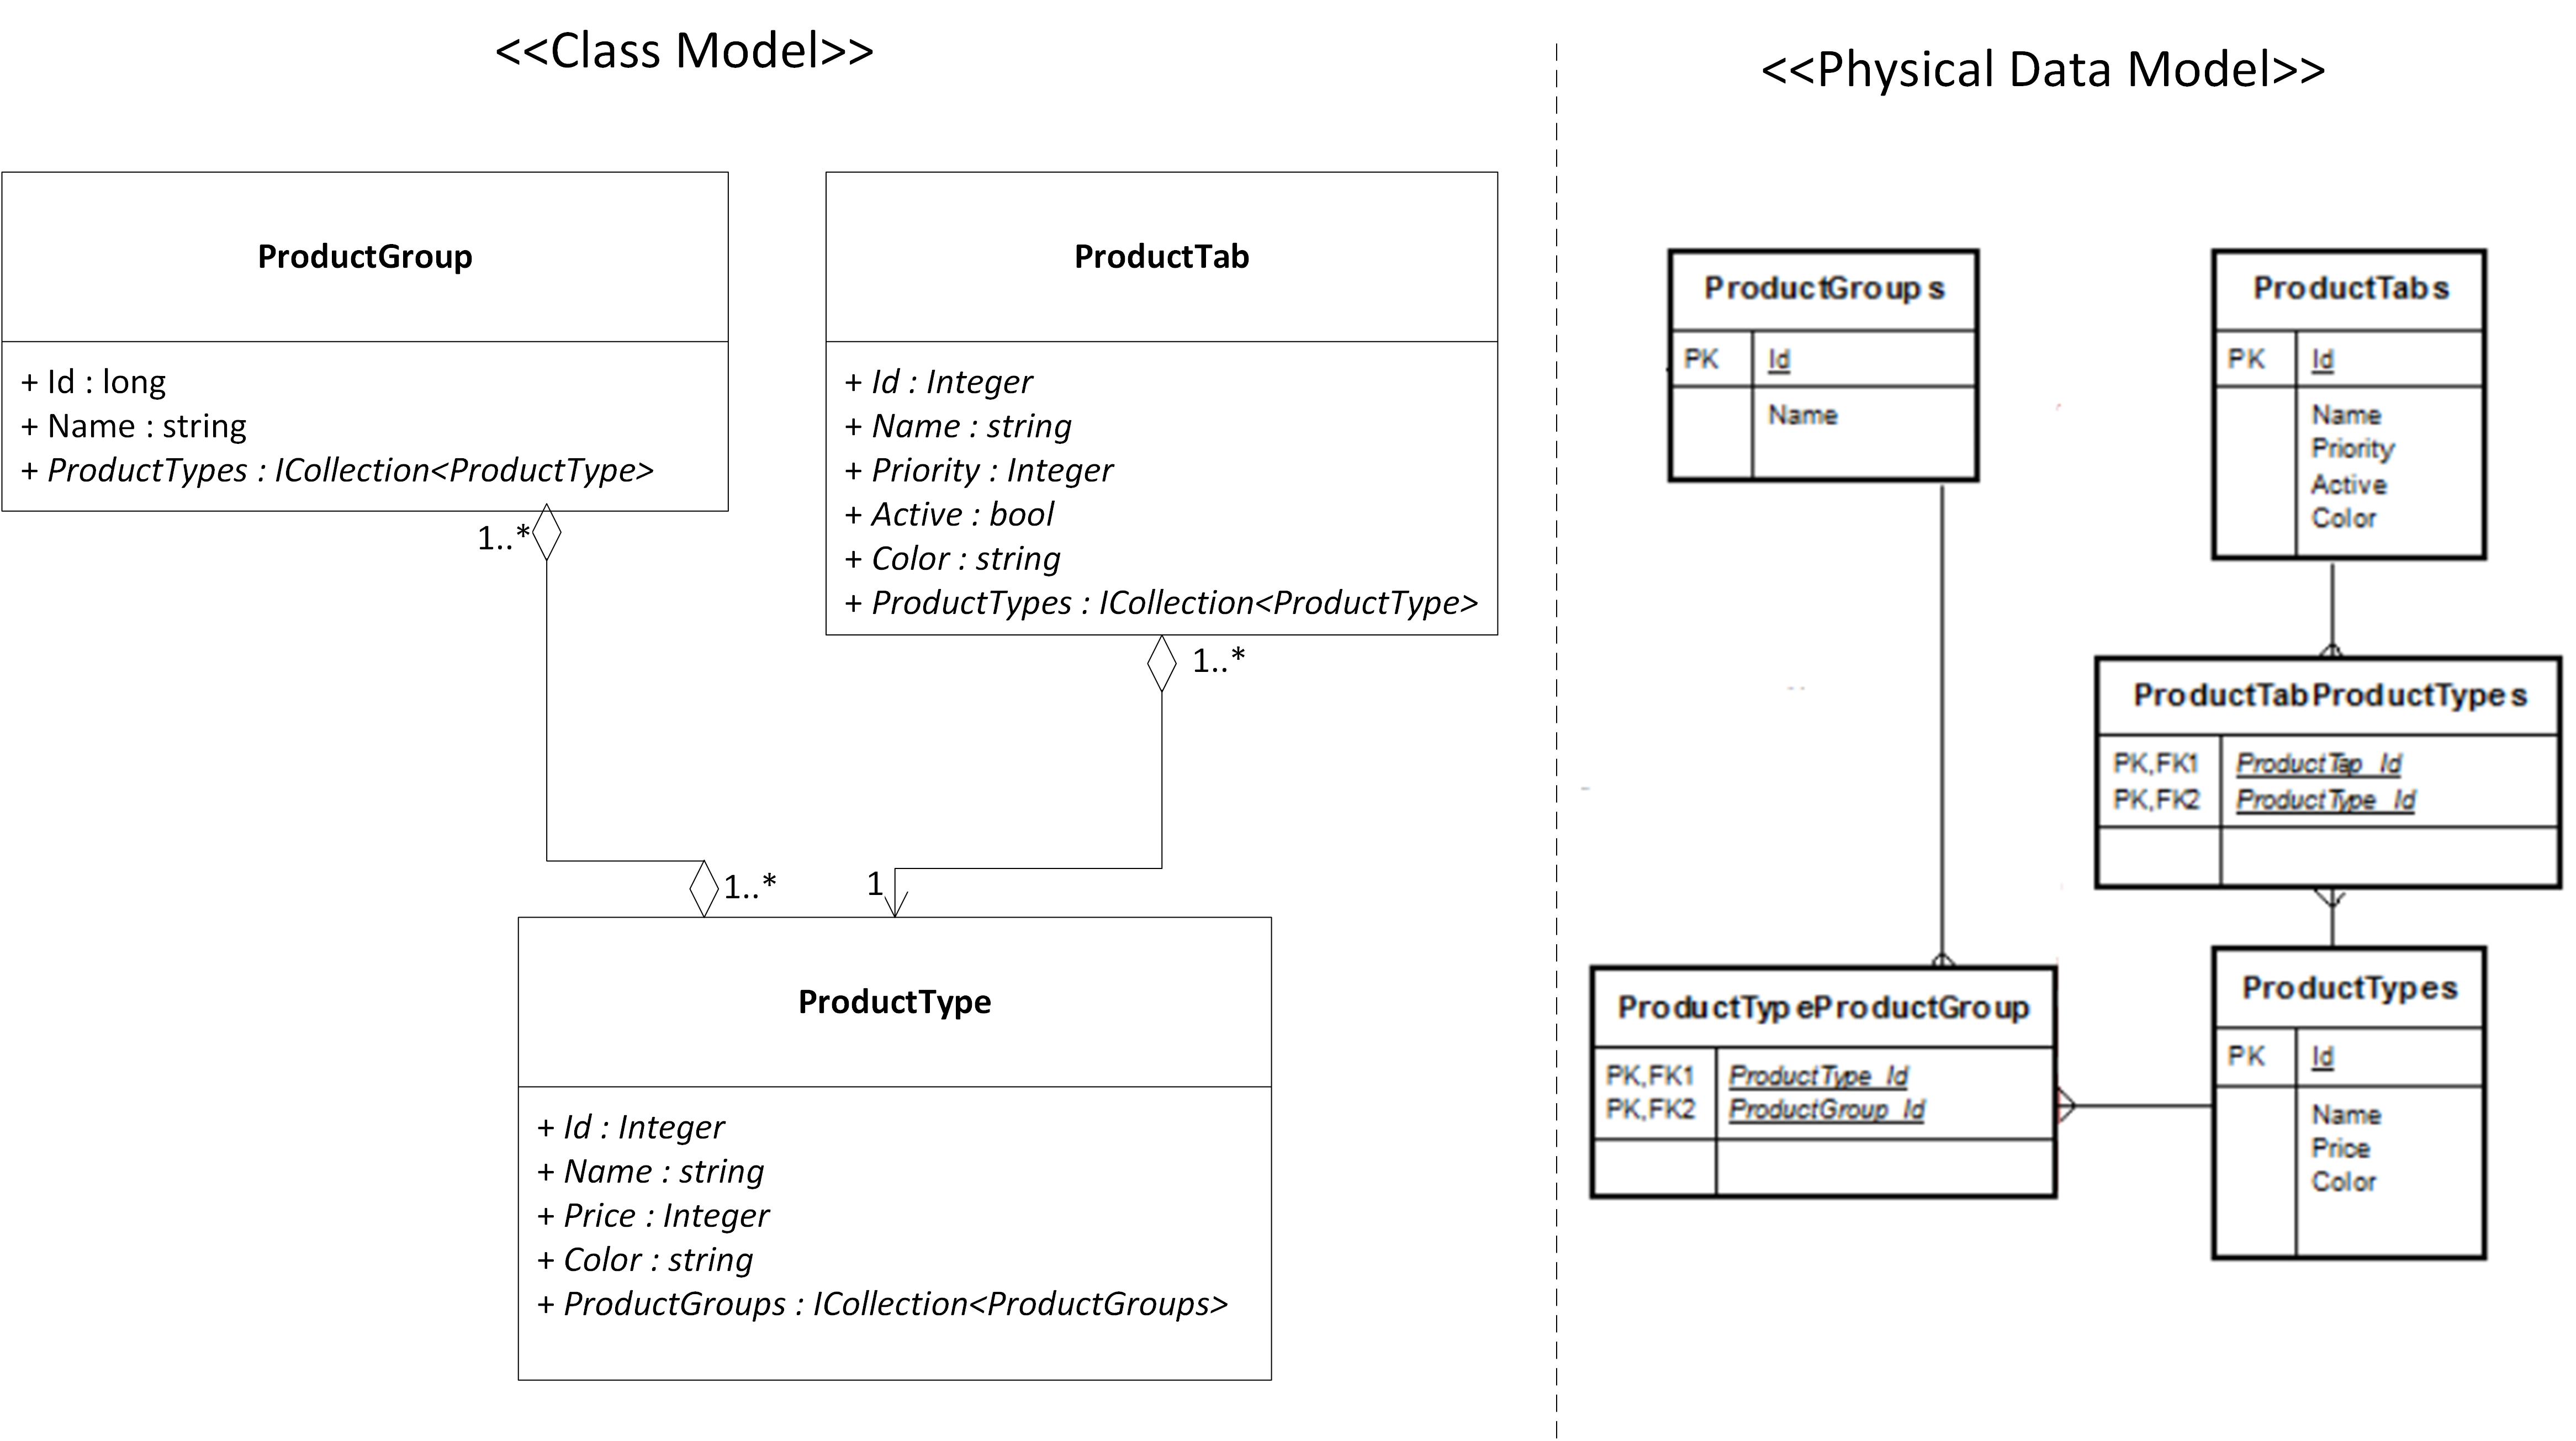
\includegraphics[width=1\textwidth]{N+1/DataView/mapping/Mapping4}
    \caption{Kobling af ProductTap og ProductType}
    \label{fig:Mapping_ProductTap_Type}
\end{figure}

ProductGroup og productType minder meget om hinanden, men ProductGroup kan fungere som undergrupper til ProductType, hvor det skal være muligt at der kan være flere productGroups under en ProductType, men en ProductGroup skal også kunne være indeholdt i flere ProductTypes derfor giver det en many-to-many tabel.
\newline
\newline
På GUI'ens knapper øverst til højre har disse deres information fra ProductTaps i database, ProductTap har et many-to-many forhold med ProductTypes, som er løst i klassemodellen ved at have en ICollection af den anden. 
